\scanpage{49}
$I$ ens ordonné

On va \unsure{interpreter|interpréter} $I^{\wedge}$ comme un $\operatorname{Top}(X)$

On a $I\simeq\operatorname{Top}(X)$ ; considérons la topologie canonique, Pour ceci, quels sont les cribles de $I$ : parties \inserted{$\sigma$} de $I$ telles que pour $\forall\ x\in\sigma$, les $y\leq x$ sont dans $\sigma$\unsure{.|,} On met sur $I$ la topologie définie par cet ens. de \deleted{cribles} parties (\deleted{\unsure{anti}}\unsure{appeler|appelle|-appeler|-appelle} la topologie des cribles) On trouve que $\deleted{\unsure{\operatorname{Top}(I|\operatorname{Top}(}}$ \unsure{l'on.|lim.}
\[
\begin{aligned}
\operatorname{Ouv}(I)&\overset{\mathrm{déf}}{=}\operatorname{Crib}(I)\simeq\operatorname{Ouv}(I^{\wedge}) \qquad\text{donc}\\
I^{\wedge}&\simeq\operatorname{Ouv}(I)^{\sim}=\operatorname{Top}(I).
\end{aligned}
\]

\uline{NB} La relation $y\leq x$ signifie que $y$ est une \uline{générisation} de $x$\\
\hspace*{3em}(non : une spécialisation)

\medskip
\noindent$\bullet$\quad $E$ a suffisamment de pts essentiels, \unsure{et est|étant} engendré par ses ouverts

\noindent\hspace*{1.6em}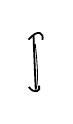
\begin{tikzpicture}[x=1em,y=1em]
\draw[line width=.65pt] (0,2.08) .. controls (.02,1.5) and (.06,.55) .. (.08,.15);
\draw[line width=.3pt] (.06,1.8) .. controls (.16,.9) and (.17,.35) .. (.08,.15);
\draw[line width=.65pt] (-.18,1.95) .. controls (.16,2.35) and (.38,2.2) .. (.32,1.94);
\draw[line width=.65pt] (-.17,.24) .. controls (.02,-.03) and (.28,.08) .. (.20,.29);
\end{tikzpicture}

\noindent\hspace*{1.6em}\begin{minipage}[t]{\dimexpr\linewidth-1.6em\relax}
$E$ est engendré par les \deleted{\unsure{objets|objet}} \unsure{sous-objet|sous-objets} de l'objet final\unsure{.} qui sont connexes, non vides et projectifs.
\end{minipage}

\noindent\hspace*{1.8em}
\begin{tikzpicture}[x=.08mm,y=-.08mm,baseline=(current bounding box.center)]\draw[line width=.5pt,line cap=round] (22,13)..controls(25,17)and(25,19)..(25,26) (25,30)..controls(26,49)and(23,80)..(26,96) (33,24)..controls(34,60)and(34,88)..(35,120);\draw[line width=1pt,line cap=round,line join=round] (24,32)--(34,20)--(37,27) (27,100)--(31,110) (24,112)..controls(27,120)and(30,120)..(35,123)--(35,108);\end{tikzpicture}

\noindent\hspace*{1.8em}\begin{minipage}[t]{\dimexpr\linewidth-1.8em\relax}
(\deleted{\unsure{où|Que}}\unsure{si|où|Ex.} $E=C^{\wedge}$) Tous les morphismes de $C$ sont des monomorphismes
\end{minipage}

\noindent\hspace*{.63\linewidth}\begin{tikzpicture}[x=1em,y=1em]
\draw[line width=.35pt] (0,.9)--(.27,.63);
\draw[line width=.5pt] (.04,.36)--(.17,.29);
\draw[line width=.5pt] (.22,.25)--(.56,0);
\draw[line width=.35pt] (.83,.37)--(.94,.25);
\draw[line width=.35pt] (1.00,.18)--(1.12,.02);
\end{tikzpicture}

\noindent\hspace*{2em}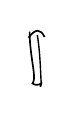
\begin{tikzpicture}[x=1em,y=1em]
\draw[line width=.6pt] (0,1.97) .. controls (.00,1.25) and (.18,.55) .. (.16,.27) .. controls (.16,.18) and (.12,.13) .. (.11,.10);
\draw[line width=.5pt] (.28,1.84) .. controls (.39,1.13) and (.39,.52) .. (.42,.10);
\draw[line width=.6pt] (-.04,1.75) .. controls (.21,2.08) and (.40,2.08) .. (.54,1.77);
\draw[line width=.6pt] (.08,.11) .. controls (.19,.02) and (.31,.03) .. (.42,.09)--(.39,-.03);
\end{tikzpicture}

\noindent\hspace*{2em}\begin{minipage}[t]{\dimexpr\linewidth-2em\relax}
(si $E=\operatorname{Top}(X)$, $X$ sobre) Pour $\forall\ x\in X$, l'ens des générisations de $x$ est\rlap{\hspace{.5em}\raisebox{-1em}{\begin{tikzpicture}[x=1em,y=1em]\draw[line width=.5pt] (0,0)--(.45,.11);\end{tikzpicture}}} un voisinage de $x$.
\end{minipage}

\noindent\hspace*{.74\linewidth}
\begin{tikzpicture}[x=1em,y=1em]
\draw[line width=.6pt] (.42,1.05)--(.54,.97);
\draw[line width=.65pt] (0,.70)--(.78,.23);
\draw[line width=.65pt] (.61,.53)--(.85,.35);
\draw[line width=.7pt] (.85,.67)--(1.00,.62);
\draw[line width=.6pt] (.48,.23)--(.66,.06);
\draw[line width=.5pt] (.89,.20)--(.95,.18);
\end{tikzpicture}\hspace{.8em}
\begin{tikzpicture}[x=.12mm,y=-.12mm,baseline=(current bounding box.center)]\draw[line width=.8pt,line cap=round,line join=round] (25,23)..controls(29,26)and(33,27)..(35,24)..controls(38,27)and(43,27)..(48,27);\draw[line width=.5pt,line cap=round] (34,39)--(53,45);\end{tikzpicture}

\vspace*{3em}
\noindent\hspace*{.94\linewidth}\begin{tikzpicture}[x=1em,y=1em]
\draw[line width=.65pt] (0,0)--(.26,.07);
\end{tikzpicture}
% archive sheet number: 48
